% PGFPlots matrix plot generated from numpy array
% Matrix size: 7x7
% Data range: [-0.744218, 1.000000]

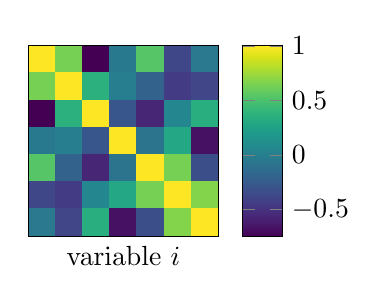
\begin{tikzpicture}
\begin{axis}[
    width=4cm,
    height=4cm,
    enlargelimits=false,
    axis equal image,
    colormap/viridis,
    xmin=-0.5, xmax=6.5,
    ymin=-0.5, ymax=6.5,
    colorbar,
    xlabel={variable $i$},
    ticks=none,
]

\addplot[
    matrix plot,
    mesh/cols=7,
    point meta=explicit
] table[meta=z] {
x y z
0 0 1.000000
1 0 0.635165
2 0 -0.744218
3 0 -0.041629
4 0 0.536644
5 0 -0.371692
6 0 -0.041931
0 1 0.635165
1 1 1.000000
2 1 0.371275
3 1 -0.001649
4 1 -0.200467
5 1 -0.437939
6 1 -0.381453
0 2 -0.744218
1 2 0.371275
2 2 1.000000
3 2 -0.279991
4 2 -0.559379
5 2 0.055969
6 2 0.346918
0 3 -0.041629
1 3 -0.001649
2 3 -0.279991
3 3 1.000000
4 3 -0.082434
5 3 0.296075
6 3 -0.671658
0 4 0.536644
1 4 -0.200467
2 4 -0.559379
3 4 -0.082434
4 4 1.000000
5 4 0.638535
6 4 -0.333148
0 5 -0.371692
1 5 -0.437939
2 5 0.055969
3 5 0.296075
4 5 0.638535
5 5 1.000000
6 5 0.675766
0 6 -0.041931
1 6 -0.381453
2 6 0.346918
3 6 -0.671658
4 6 -0.333148
5 6 0.675766
6 6 1.000000
};

\end{axis}
\end{tikzpicture}
